\documentclass[11pt]{beamer}
\setbeamertemplate{navigation symbols}{}
\geometry{paperwidth=31cm,paperheight=15cm}

\setbeamersize{text margin left=15pt,text margin right=2cm, sidebar width left=0pt,sidebar width right=10pt,}

\usepackage{mathtools}

\usepackage{tikz}
\usetikzlibrary{positioning,arrows}
\usepackage{stackengine}
\usetikzlibrary{tikzmark,fit,backgrounds,mindmap,decorations.text,shapes.callouts,arrows}
\usetikzlibrary{arrows, chains,through, positioning, trees, shapes.symbols}
\usetikzlibrary{arrows.meta}
%\usetikzlibrary{shadows}
\usetikzlibrary{shadings}
%% even fancier shadows
%\usetikzlibrary{shadows.blur}
\usetikzlibrary{fadings}
%\usepackage[english]{babel}

\usepackage{physics}
\usepackage{graphicx}
%\usepackage{ragged2e}
%\usepackage[most]{tcolorbox}
%\usepackage{mdframed}

%%%%%%%%%%%%%%%%%%equation highlighter%%%
\tikzset{every picture/.style={remember picture}}
%%%%%%%%%%%%%%%%%%%%%%%

\begin{document}
	\begin{frame}
	
	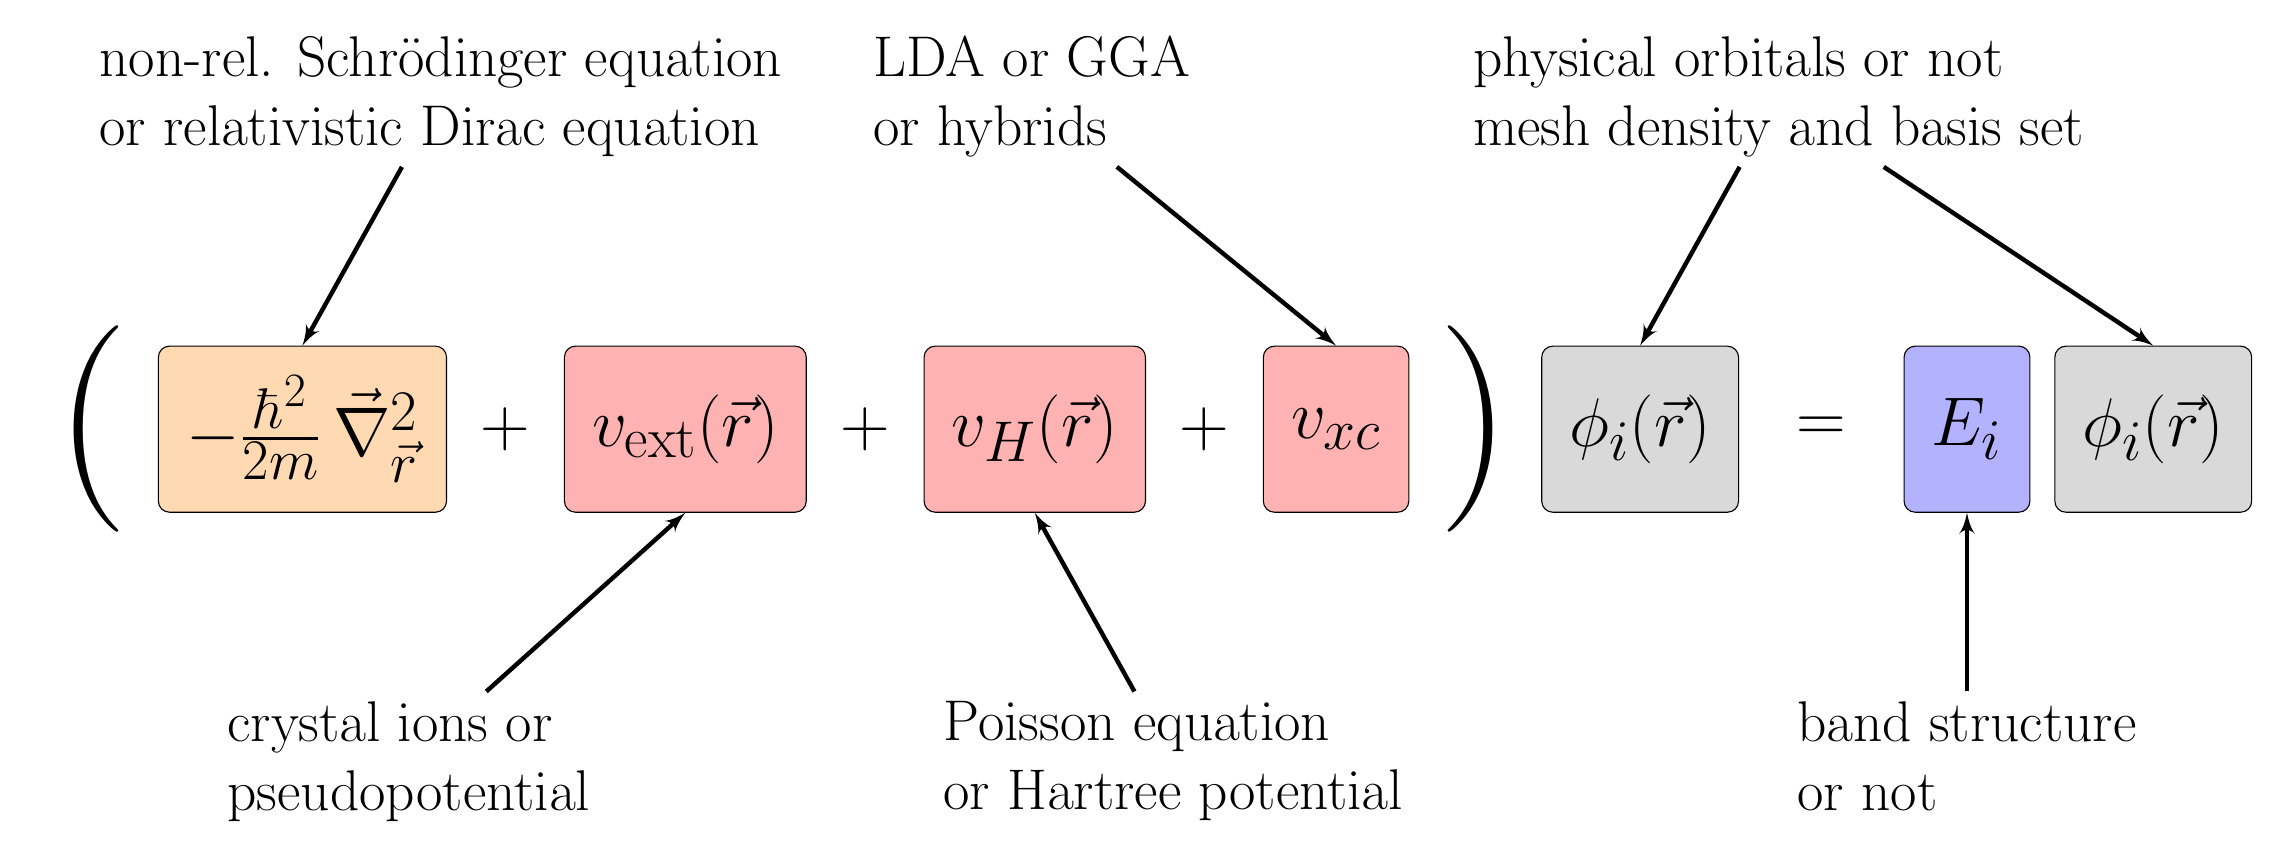
\begin{tikzpicture}[
		g/.style={rectangle,draw,rounded corners,minimum height=6em,inner sep=1em,font=\Huge},
		w/.style={font=\Huge},
		c/.style={node distance=15ex,align=left,font=\huge},
		a/.style={draw,-latex',ultra thick}
		]
		
		\node [w,scale=3] (bra) {(};
		\node [node distance=0ex,fill=orange!30,g,right=of bra] (kinetic) {$-\frac{\hbar^2}{2m}\,\vec{\nabla}_{\vec{r}}^2$};
		\node [node distance=2ex,w,right=of kinetic] (plus1) {$+$};
		\node [node distance=2ex,fill=red!30,g,right=of plus1] (external) {$v_\text{ext}(\vec{r})$};
		\node [node distance=2ex,w,right=of external] (plus2) {$+$};
		\node [node distance=2ex,fill=red!30,g,right=of plus2] (hartree) {$v_H(\vec{r})$};
		\node [node distance=2ex,w,right=of hartree] (plus3) {$+$};
		\node [node distance=2ex,fill=red!30,g,right=of plus3] (xc) {$v_{xc}$};
		\node [node distance=0ex,w,right=of xc,scale=3] (ket) {)};
		\node [node distance=0ex,fill=gray!30,g,right=of ket] (phi1) {$\phi_i(\vec{r})$};
		\node [node distance=4ex,w,right=of phi1] (equal) {$=$};
		\node [node distance=4ex,fill=blue!30,g,right=of equal] (energy) {$E_i$};
		\node [node distance=2ex,fill=gray!30,g,right=of energy] (phi2) {$\phi_i(\vec{r})$};
		
		\node [c,above=of kinetic,xshift=5em] (kinetic comment) {non-rel. Schr\"{o}dinger equation\\or relativistic Dirac equation};
		\node [c,below=of external,xshift=-10em] (external comment) {crystal ions or\\pseudopotential};
		\node [c,below=of hartree,xshift=5em] (hartree comment) {Poisson equation\\or Hartree potential};
		\node [c,above=of xc,xshift=-11em] (xc comment) {LDA or GGA\\or hybrids};
		\node [c,above=of phi1,xshift=5em] (phi comment) {physical orbitals or not\\mesh density and basis set};
		\node [c,below=of energy] (energy comment) {band structure\\ or not};
		
		\path [a] (kinetic comment) -- (kinetic.north);
		\path [a] (external comment) -- (external.south);
		\path [a] (hartree comment) -- (hartree.south);
		\path [a] (xc comment) -- (xc.north);
		\path [a] (phi comment) -- (phi1.north);
		\path [a] (phi comment) -- (phi2.north);
		\path [a] (energy comment) -- (energy.south);
		
	\end{tikzpicture}
		\end{frame}
		
		%%%%%%%%%%%%%%%%%%%%%%%%%%%%%%%%%%%%%%%%%%%%%%%%%
	\begin{frame}
		\centering
		\Huge
		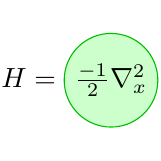
\begin{tikzpicture}
			$H= \tikz[baseline]{ 
				\node	(d1)  at (0.0,0.0) [draw=green!75!black,fill=green!20,anchor=base,circle,inner sep = 2pt]
				{$\frac{-1}{2}\laplacian_{x}$};}+
			\tikz[baseline]{ 
				\node(d2)  at (1,0) [draw=red,fill=red!20,ultra thick, anchor=base, circle, inner sep = 5pt]
				{V(x)}; } $;
		\end{tikzpicture}%
		\begin{tikzpicture}[overlay,scale=2]
			\draw[blue,ultra thick,->>] (d1) to [bend left] +(70:2cm) node[anchor=west,text = black, align = left] {Kinetic Energy};
			
			\draw[orange,ultra thick,->>] (d2) -- ++(30:70pt) node[anchor=west,text = blue, align = left] {\textbf{ Potential}};
		\end{tikzpicture}
	\end{frame}
	%%%%%%%%%%%%%%%%%%
	
	\begin{frame}
		\Huge
		\begin{equation*}
			\hat{A}(t) =
			\underbrace{e^{\frac{iHt}{\hbar}}}_{\color{blue}
				\text{\fbox{\parbox[b]{1cm}{\tiny\raggedright\color{black}Backward}}}
			}
			\underbrace{\hat{A}}_{\color{red}
				\text{\fbox{\parbox[b]{1.4cm}{\tiny\raggedright\color{black}Perturbation}}}
			}
			\underbrace{e^{\frac{-iHt}{\hbar}}}_{\color{green!75!black}
				\text{\fbox{\parbox[b]{0.8cm}{\tiny\raggedright\color{black}Forward}}}
			}
		\end{equation*}
	\end{frame}
	
	%%%%%%%%%%%%%%%%%%%%%%%%%%%%%%%%%%%%%
			\begin{frame}
				\Huge
		\begin{equation*}
			\hat{\mathcal{H}}\psi(x) = 
			\underbrace{\left( -\frac{1}{2}\laplacian_x - \frac{1}{2}\hat{x}^2 \lambda \right)\psi(x)}_{\color{red}
				\begin{tabular}{c}
					\text{Scattering off a}\\
					\text{parabolic potential barrier}
				\end{tabular}
			} = E\psi(x)
		\end{equation*}
		
	\end{frame}
	
	%%%%%%%%%%%%%%%%%%%%%%%%%%%%%%%%%%%%%%%%%%%%%%%%%%%%%%%%%%%%%%%%%%%%%
	\begin{frame}
		\Huge
		\begin{equation*}
			\mathcal{H}=\frac{\hat{p}^2}{2}\; \tikz[baseline]{\node[draw=red, ultra thick,anchor=base,rectangle,rounded corners,inner sep = 3pt](d12) {$-$};} \frac{1 }{2}\hat{x}^2\; \tikz[baseline]{\node[draw=red, ultra thick,anchor=base,rectangle,rounded corners,inner sep = 3pt](d11) {$\lambda$};}
		\end{equation*}	
		\begin{tikzpicture}[overlay,remember picture]
			\draw[red,ultra thick,->] (d12) -- +(270:3cm) node[anchor=north, text = red, align = right] {Inversion};
			\draw[red,ultra thick,->] (d11) -- +(350:2.8cm) node[anchor=north,text = red,align = right] {Curvature of \\ the potential};
			% 
		\end{tikzpicture}
		
		
	\end{frame}
\end{document}
